%& -shell-escape -enable-write18
%Preample: \pgfplotsset{width=7cm,compat=1.3}:
\documentclass{standalone}
\usepackage{tikz}
\usepackage{pgfplots}
%\pgfplotsset{compat=1.3}
%\usepackage{caption}
\usetikzlibrary{external}
\usetikzlibrary{shapes,arrows}
%\newcommand{mynodename}[#1]{\mathrm{#1}}
%\newcommand{mylabelleft}[#2]{label={[font=\fontsize{#1}{#1}\selectfont]above left:mynodename{#2}}}
\begin{document}

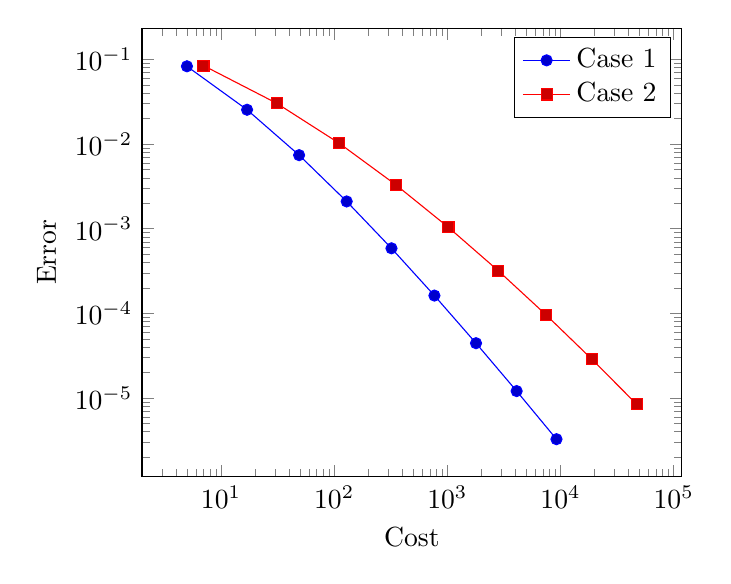
\begin{tikzpicture}
\begin{loglogaxis}[xlabel=Cost,ylabel=Error]
\addplot coordinates {
(5, 8.31160034e-02)
(17, 2.54685628e-02)
(49, 7.40715288e-03)
(129, 2.10192154e-03)
(321, 5.87352989e-04)
(769, 1.62269942e-04)
(1793, 4.44248889e-05)
(4097, 1.20714122e-05)
(9217, 3.26101452e-06)
};
\addplot coordinates {
(7, 8.47178381e-02)
(31, 3.04409349e-02)
(111, 1.02214539e-02)
(351, 3.30346265e-03)
(1023, 1.03886535e-03)
(2815, 3.19646457e-04)
(7423, 9.65789766e-05)
(18943, 2.87339125e-05)
(47103, 8.43749881e-06)
};
\legend{Case 1,Case 2}
\end{loglogaxis}
\end{tikzpicture}

\pgfplotsset{footnotesize,samples=10}
\begin{centering}% note that \centering uses less vspace...
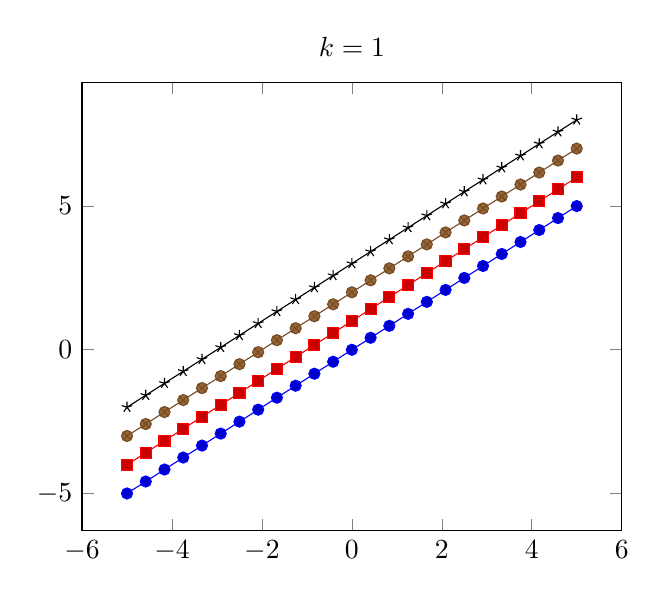
\begin{tikzpicture}
\begin{axis}[
legend columns=-1,
legend entries={$(x+0)^k$;,$(x+1)^k$;,$(x+2)^k$;,$(x+3)^k$},
legend to name=named,
title={$k=1$}]
\addplot {x};
\addplot {x+1};
\addplot {x+2};
\addplot {x+3};
\end{axis}
\end{tikzpicture}
%
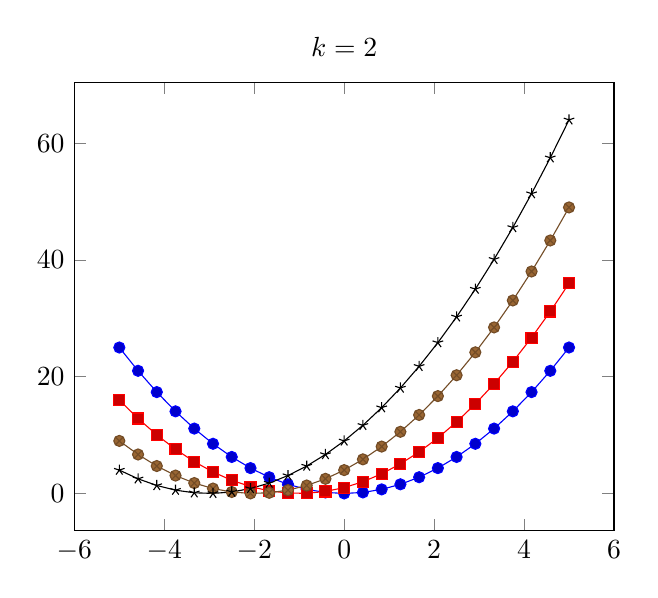
\begin{tikzpicture}
\begin{axis}[title={$k=2$}]
\addplot {x^2};
\addplot {(x+1)^2};
\addplot {(x+2)^2};
\addplot {(x+3)^2};
\end{axis}
\end{tikzpicture}
%
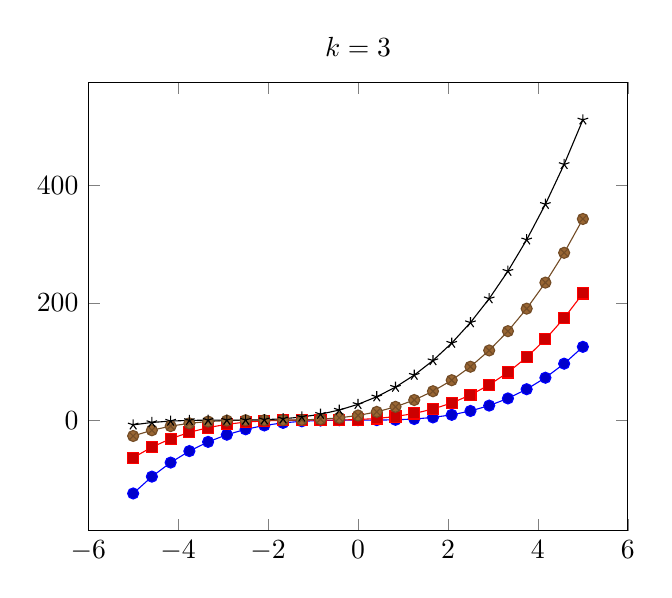
\begin{tikzpicture}
\begin{axis}[title={$k=3$}]
\addplot {x^3};
\addplot {(x+1)^3};
\addplot {(x+2)^3};
\addplot {(x+3)^3};
\end{axis}
\end{tikzpicture}
\\
\ref{named}
\end{centering}

\begin{tikzpicture}
\begin{loglogaxis}[
xlabel=Dof,
ylabel=$L_2$ error]
\addplot table[x=dof,y=L2] {datafile.dat};
\end{loglogaxis}
\end{tikzpicture}
\end{document}
